\documentclass[12pt,letterpaper]{article}
\usepackage{fullpage}
\usepackage[top=1.5cm, bottom=3.5cm, left=2.2cm, right=2.2cm]{geometry}
\usepackage{amsmath,amsthm,amsfonts,amssymb,amscd, esint}
\usepackage{lastpage}
\usepackage{enumerate}
\usepackage{fancyhdr}
\usepackage{mathrsfs}
\usepackage{graphicx}
\usepackage{listings}
\usepackage{hyperref}
\usepackage[english]{babel}
\usepackage{lipsum}
\usepackage[table,xcdraw]{xcolor}
\usepackage{enumitem}
\usepackage{float}
\usepackage{chemfig}
\usepackage{yfonts}
\usepackage{braket}
\usepackage{dsfont}
\usepackage{tikz}
\usepackage{wrapfig}
\usepackage{url}
\usepackage{natbib}
\usepackage[normalem]{ulem}
\usepackage{multicol}
\useunder{\uline}{\ul}{}


%%%%%%%%%%%%%%% CODELISTINGS %%%%%%%%%%%%%%%%
\usepackage{listings}
\definecolor{codegreen}{rgb}{0,0.6,0}
\definecolor{codegray}{rgb}{0.5,0.5,0.5}
\definecolor{codepurple}{rgb}{0.58,0,0.82}
\definecolor{backcolour}{rgb}{0.95,0.95,0.92}

\lstdefinestyle{mystyle}{
    backgroundcolor=\color{backcolour},   
    commentstyle=\color{codegreen},
    keywordstyle=\color{magenta},
    numberstyle=\tiny\color{codegray},
    stringstyle=\color{codepurple},
    basicstyle=\ttfamily\footnotesize,
    breakatwhitespace=false,
    breaklines=true,                 
    captionpos=t,                    
    keepspaces=true,                 
    numbers=left,                    
    numbersep=5pt,                  
    showspaces=false,                
    showstringspaces=false,
    showtabs=false,                  
    tabsize=2
}

\lstset{style=mystyle}

%%%%%%%%%%%%%%%%%%%%%%%%%%%%%%%%%%%%%%% 
\usepackage{titlesec}
\usepackage{textcase} % for uppercase handling

% --- Section formatting ---
\titleformat{\section}
  {\normalfont\normalsize\bfseries\centering} % font size, bold, centered
  {\thesection}{1em}{\MakeTextUppercase} % uppercase text

% --- Subsection formatting ---
\titleformat{\subsection}
  {\normalfont\normalsize\bfseries\centering}
  {\thesubsection}{1em}{\MakeTextUppercase}

% --- Roman numerals for numbering ---
\renewcommand{\thesection}{\Roman{section}}
\renewcommand{\thesubsection}{\Roman{section}.\Roman{subsection}}

\newtheorem{definition}{Definition}
\newtheorem{observation}{Observation}
\newtheorem{reflection}{Reflection}
\newtheorem{PyPackage}{Package}
\newtheorem{book}{Book}

\newcommand{\HRule}[1]{\rule{\linewidth}{#1}}
\setcounter{tocdepth}{5}
\setcounter{secnumdepth}{5}

%\setlength{\parindent}{0.0in}
%\setlength{\parskip}{0.05in}

% Edit these as appropriate
\newcommand\course{}
\newcommand\subject{Final Degree Project}
\newcommand\degree{Bachelor's Degree in Physics}
\newcommand\documenttitle{Lower bounds of the success probability in quantum state exclusion for general ensembles}
\newcommand\NetIDb{Universitat Autònoma de Barcelona}
\newcommand\AuthorName{Sergio Castañeiras Morales}

\hypersetup{%
  pdftitle  = \documenttitle,
  pdfauthor = \AuthorName,
  pdfsubject= \degree,
  pdfcreator= \AuthorName,
  hidelinks = true,
}

\usepackage{glossaries}
\usepackage{glossary-longragged}

\makenoidxglossaries
\newacronym{qse}{QSE}{Quantum State Exclusion}
\newacronym{qsd}{QSD}{Quantum State Discrimination}
\newacronym{sdp}{SDP}{Semidefinite Program}
\newacronym{povm}{POVM}{Positive Operator-Valued Measure}
\newacronym{me}{ME}{Minimum Error}
\newacronym{ze}{ZE}{Zero Error}
\glsaddall[types=\acronymtype] 

\DeclareMathOperator{\tr}{Tr}
\usetikzlibrary{arrows.meta, positioning}

\begin{document}
\title{\vspace{4cm} \normalsize 
		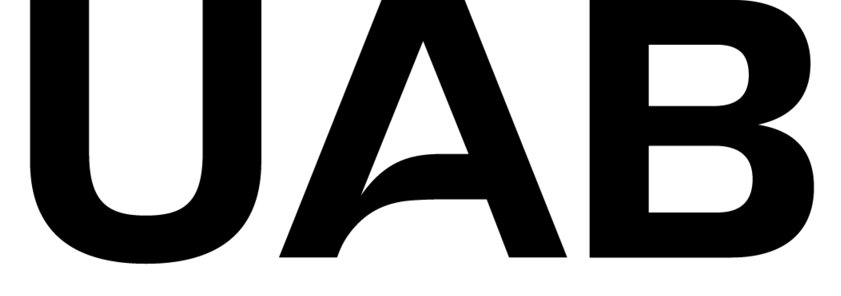
\includegraphics[width = 0.25\textwidth]{GeneralSources/UABLogo.png}\\ [0.5cm]
		\textsc{\NetIDb}\\ [2.0cm]
		\HRule{0.5pt} \\
		\LARGE \textbf{\uppercase{\documenttitle}}
		\HRule{2pt} \\ [1.5cm]
		\normalsize \begin{tabular}{rcl}  % Create a right-left column alignment
        \textsc{Author} & : & \textsc{\AuthorName} \\
        \textsc{Supervisor} & : & \textsc{Ramón Muñoz Tapia} \\
        \textsc{Co-Supervisor} & : & \textsc{Santiago Llorens Fernández}
    \end{tabular}
    \normalsize \vspace*{5\baselineskip}
		}

\date{2024-2025}

\author{\large \textsc{\subject} \\ \textsc{\degree}}



\begin{titlepage}
\clearpage\maketitle
\thispagestyle{empty}
\end{titlepage}

\thispagestyle{empty}
\mbox{} 
\newpage
\thispagestyle{empty}
\vspace*{\fill} % Push content to vertical center
\begin{flushright}
    \emph{Ab ovo usque ad mala.}\\[1em]
    \textbf{Horace}
\end{flushright}
\vspace*{\fill} 
\newpage

\newpage
\pagestyle{fancyplain}
\headheight 35pt
\lhead{\NetIDb}    
\rhead{\subject}
\cfoot{\small\thepage}
\headsep 1.5em
\setcounter{page}{1}
\begin{multicols}{2}[\begin{center}
\begin{abstract}
Given a quantum state known to be prepared from an ensemble of two or more states, quantum state exclusion aims to rule out the possibility that it was prepared in a particular state from the ensemble. Using the known solution for group generated ensembles \cite{MainPaper}, we study this result as a lower bound for randomly generated ensembles via semidefinite programming.
\end{abstract}
\end{center}
Keywords: \emph{SDP, Quantum state exclusion , \textcolor{blue}{Add keywords}}.
]
\section{Introduction}
In many real-world scenarios, excluding a certain hypothesis can be more practical than solving the problem entirely. For instance, in disease diagnosis, ruling out potential diseases often serves as the first step in identifying the actual condition. Similarly, when repairing a machine, it is sometimes more efficient to identify the components that are functioning correctly, which narrows down the search for the faulty part.

In this project, we project this idea into the quantum realm by focusing on \gls{qse}. Rather than determining the exact state of a quantum system, we aim to eliminate one or more possible candidates from a known ensemble of states. Notice, this approach can be more suitable or efficient in certain quantum information tasks.

Given a quantum state known to be prepared from a finite ensemble, \gls{qsd} seeks to identify which specific state from the ensemble corresponds to the given system. In contrast, \gls{qse}~\cite{PhysicsExclusionSource} adopts the opposite perspective: it aims to determine which states from the ensemble do not correspond to the prepared state. While \gls{qsd} has been deeply studied in recent years\cite{DiscriminationArticle}, with significant advances since its inception~\cite{helstromBook}, \gls{qse} offers a complementary framework with distinct advantages.

Although the tasks of exclusion and discrimination coincide for ensembles containing only two states \footnote{Since for the two states case excluding one necessarily implies identifying the other.}, when dealing with ensembles of three or more states, the two problems diverge in both approach and complexity. One of the most significant features of \gls{qse} is the possibility of achieving \emph{perfect exclusion}, where certain states can be ruled out with zero probability of error in cases where \emph{perfect discrimination} is impossible\cite{OptimalitySRM}. 

This capability opens new frontiers in quantum information theory, particularly in the context of partial information retrieval from quantum systems. By excluding certain states, it is possible to gain insight into the encoded information without needing to fully determine the original state.

As with \gls{qsd}, obtaining a general analytical solution for \gls{qse} remains an open problem. However, analytical results have been found in specific cases when the ensemble of quantum states exhibits a certain degree of symmetry. In particular, when the ensemble is generated by the action of a finite group, the problem becomes more tractable and exact solutions have been derived.

The exclusion task can be carried out under two main protocols: \gls{me} and \gls{ze}\footnote{Also known as \emph{unambiguous exclusion}.}. In the Minimum Error scenario, the goal is to minimize the probability of mistakenly excluding the actual prepared state. In contrast, the Zero Error approach seeks to exclude a state with absolute certainty, even if that means sometimes the procedure yields an inconclusive result.

Building on recent results that provide exact solutions for exclusion tasks in group generated ensembles \cite{MainPaper}, this project undertakes a numerical study of such results as lower bounds for more general, randomly generated ensembles. To this end, we employ \gls{sdp} to explore \gls{qse} performance in arbitrary settings. Furthermore, we investigate improved bounds for the general case based on how closely a given ensemble resembles a group generated one\footnote{The notion of "how close" will be formally defined in Section~\textcolor{blue}{add section}.}.

\subsection{Formulation of the Problem}

Let $\left\{(\rho_i, \eta_i)\right\}_{i=1}^n$ be an ensemble of $n$ quantum states, where each $\rho_i$ denotes a pure state density matrix\footnote{This formulation hols true for mixed states but the project will only discuss the pure state scenario.}, i.e., $\rho_i = \ket{\psi_i}\bra{\psi_i}$, and $\eta_i$ represents the prior probability of occurrence of the state $\rho_i$. Let $\rho_j$ be the target state from this ensemble. Our objective is to develop a procedure to identify another state $\rho_k \in \left\{\rho_i\right\}_{i=1}^n$, such that $\rho_k \neq \rho_j$.

Quantum measurements are described by a set of \glspl{povm}, denoted by $\left\{\Pi_i\right\}_{i=1}^n$, acting on the Hilbert space $\mathcal{H}$ of the quantum system. Here we pewsent the two studied protocols for \gls{qse}: minimum-error (\gls{me}) and zero-error (\gls{ze}).

The goal of the \gls{me} protocol is to minimize the probability of incorrectly excluding the target state from our hypothesis. If we formulate it as an \gls{sdp}, the problem reads,\footnote{Note that the \gls{sdp} formulations of quantum state discrimination may differ from the exclusion ones by interchanging minimization and maximization problems.}
\begin{align*}
	P_{\text{\gls{me}}}^e = \min_{\left\{\Pi_i\right\}} &\sum_{i=1}^n \tr(\Pi_i \rho_i),\\
	\text{subject to} \quad & \sum_{i=1}^n \Pi_i = \mathds{1}, \quad \Pi_i \geq 0 \quad \forall i \in \{1, \dots, n\}.
\end{align*}

Note the constraints $\sum_{i=1}^n \Pi_i = \mathds{1}$ and $\Pi_i \geq 0$ ensure that the $\Pi_i$ form a valid POVM, since they demand positive semi-definition and form a complete measurement. The superscript $e$ in $P_{\text{\gls{me}}}^e$ indicates that this is the \emph{error probability}.

Alternatively, we may formulate the problem in terms of the \emph{success probability}, denoted by $P_{\text{\gls{me}}}^s$, which quantifies the probability of a correct exclusion. This equivalent formulation reads,
\begin{align*}
	P_{\text{\gls{me}}}^s = \max_{\left\{\Pi_i\right\}} &\left(1 - \sum_{i=1}^n \tr(\Pi_i \rho_i)\right),\\
	\text{subject to} \quad & \sum_{i=1}^n \Pi_i = \mathds{1}, \quad \Pi_i \geq 0 \quad \forall i \in \{1, \dots, n\}.
\end{align*}

Naturally, both formulations are related via:
\begin{align*}
P_{\text{\gls{me}}}^s + P_{\text{\gls{me}}}^e = 1.
\end{align*}

In the case of the \gls{ze} protocol, the POVMs must also satisfy an unambiguity condition, i.e. each measurement operator $\Pi_i$ must be orthogonal to the corresponding state $\rho_i$. In other words,
\begin{align*}
\tr(\Pi_i \rho_i) = 0 \quad \forall i \in \{1, \dots, n\}.
\end{align*}

To ensure completeness, we introduce an additional POVM element $\Pi_?$ representing an inconclusive result,
\begin{align*}
\Pi_? = \mathds{1} - \sum_{i=1}^n \Pi_i.
\end{align*}
If the measurement yields the outcome $\Pi_?$ (i.e., the "?" symbol), the result is inconclusive.

The corresponding \gls{sdp} for minimizing the probability of an inconclusive result (i.e., error) in the \gls{ze} protocol is:
\begin{align*}
	P_{\text{\gls{ze}}}^e = \min_{\left\{\Pi_i\right\}} &\sum_{i=1}^n \tr(\Pi_? \rho_i),\\
	\text{subject to} \quad & \sum_{i=1}^n \Pi_i + \Pi_? = \mathds{1}, \quad \Pi_? \geq 0,\\
	& \tr(\Pi_i \rho_i) = 0, \quad \Pi_i \geq 0 \quad \forall i.
\end{align*}

The corresponding success probability is naturally given by,
\begin{align*}
	P_{\text{\gls{ze}}}^s = \max_{\left\{\Pi_i\right\}} &\left(1 - \sum_{i=1}^n \tr(\Pi_? \rho_i)\right),\\
	\text{subject to} \quad & \sum_{i=1}^n \Pi_i + \Pi_? = \mathds{1}, \quad \Pi_? \geq 0,\\
	& \tr(\Pi_i \rho_i) = 0, \quad \Pi_i \geq 0 \quad \forall i.
\end{align*}

This formulation is analogous to the \gls{me} protocol, with the crucial difference being the constraint $\tr(\Pi_i \rho_i) = 0$, enforcing unambiguous discrimination.

\subsection{Gram matrix formulation}
Let $\mathcal{G} \in \mathbb{C}^{n \times n}$ be the \emph{Gram matrix} of the system, defined as the $n\times n$ positive semidefinite hermitian matrix such that,
\begin{equation*}
	\mathcal{G} =
	\begin{pmatrix}
		\braket{\psi_1|\psi_1} & \braket{\psi_1|\psi_2} & \dots & \braket{\psi_1|\psi_n}\\
		\braket{\psi_2|\psi_1} & \braket{\psi_2|\psi_2} & \dots & \braket{\psi_2|\psi_n}\\
		\vdots & \vdots & \ddots & \vdots\\
		\braket{\psi_n|\psi_1} & \braket{\psi_n|\psi_2} & \dots & \braket{\psi_n|\psi_n}
	\end{pmatrix},
\end{equation*}
i.e., $\mathcal{G}_{i,j} = \braket{\psi_i|\psi_j}$. Since all states are normalized, we have,
\begin{equation*}
	\mathcal{G} =
	\begin{pmatrix}
		1 & \braket{\psi_1|\psi_2} & \dots & \braket{\psi_1|\psi_n}\\
		\braket{\psi_2|\psi_1} & 1 & \dots & \braket{\psi_2|\psi_n}\\
		\vdots & \vdots & \ddots & \vdots\\
		\braket{\psi_n|\psi_1} & \braket{\psi_n|\psi_2} & \dots & 1
	\end{pmatrix}.
\end{equation*}

Notice this matrix is Hermitian by construction,
\begin{align*}
\mathcal{G}_{i,j}^* = (\braket{\psi_i|\psi_j})^* = \braket{\psi_j|\psi_i} = \mathcal{G}_{j,i}.
\end{align*}

The Gram matrix allows us to reframe the exclusion problem in a more abstract and basis-independent form. Since $\mathcal{G}$ is hermitian and positive semi-definite, we can write,
\begin{align*}
\mathcal{G} = X^\dagger X,
\end{align*}
for some matrix $X$ whose columns are the pure states,
\begin{align*}
	X = \begin{pmatrix}
		\mid & \mid &        & \mid \\
		\ket{\psi_1} & \ket{\psi_2} & \dots & \ket{\psi_n} \\
		\mid & \mid &        & \mid
	\end{pmatrix}.
\end{align*}
Notice the diagonal elements of $X$ are,
\begin{align*}
	X_{i,i}=\braket{\omega_i|\psi_i}
\end{align*}
For an arbitrary orthonormal basis $\left\{\ket{\omega_i}\right\}_{i=1}^n$. \footnote{It is important to remark that fixing the basis $\left\{\ket{\omega_i}\right\}_{i=1}^n$ fixes the decomposition of $G=X^\dagger X$ and vice versa.}

Let us consider an arbitrary orthonormal basis $\left\{\ket{\omega_i}\right\}_{i=1}^n$, and define the POVM elements as projectors $\Pi_i = \ket{\omega_i}\bra{\omega_i}$. Then, the \gls{sdp} formulation for the ensamble $\left\{(\rho_i,\eta_i)\right\}_{i=1}^n$ can be expressed as the following,
\begin{align*}
	\tr(\Pi_i \rho_i) &= \tr\left( \ket{\omega_i}\bra{\omega_i} \ket{\psi_i}\bra{\psi_i} \right) \\
	&= |\braket{\omega_i|\psi_i}|^2 \\
	&= |X_{i,i}|^2.
\end{align*}

Therefore, we can reformulate the \gls{sdp} for the \gls{me} protocol as,
\begin{align*}
	P_{\gls{me}}^e = \min_{X} &\sum_{i=1}^n \frac{|X_{i,i}|^2}{\eta_i},\\
	\text{subject to} \quad & X^\dagger X = \mathcal{G}, \quad X \geq 0.
\end{align*}

Similarly, the success probability becomes, 
\begin{align*}
	P_{\gls{me}}^s = \max_{X} &\left(1 - \sum_{i=1}^n \frac{|X_{i,i}|^2}{\eta_i}\right),\\
	\text{subject to} \quad & X^\dagger X = \mathcal{G}, \quad X \geq 0.
\end{align*}

This reformulation highlights that if two ensembles $A$ and $B$ share the same Gram matrix, then their exclusion problems, in both \gls{me} and \gls{ze} protocols, are equivalent. That is, the optimal success and error probabilities are identical in both systems. Hence, we focus on the Gram matrix to analyze exclusion problems, rather than relying on explicit state representations.

Moreover, we remark we are not especially interested in the arbitrary prior probabilities $\eta_i$ scenario, since the result for equal prior probabilities $\eta_i=\frac{1}{n}$ can be easily extended to the previous case, with $n$ as the number of states. This extension can be performed by considering the non-normalized states
\begin{align*}
	\ket{\tilde{\psi_i}}=\frac{1}{\sqrt{\eta_i}}\ket{\psi_i}
\end{align*}
and reformulate the problem in terms of this new states forgetting about the prior probabilities since they are encoded inside the states. Thus, for simplicity we will consider the equal probabilities case.

\subsection{Group Generated Ensembles}

Given a quantum state $\ket{\psi}$, which we refer to as the \emph{seed state}, we define a \emph{group generated ensemble} as the set of states obtained by applying a group of unitary transformations to $\ket{\psi}$. Specifically, if the ensemble consists of a total of $n$ quantum states, then its elements are of the form,
\begin{align*}
	U_i\ket{\psi}, \quad i \in \{1, \dots, n\},
\end{align*}
where the set of unitary matrices $\{U_i\}_{i=1}^n$ forms a finite group under standard matrix product. In terms of density matrices, the ensemble can equivalently be written as:
\begin{align*}
	\rho_i = U_i \rho U_i^\dagger, \quad i \in \{1, \dots, n\},
\end{align*}
where $\rho = \ket{\psi}\bra{\psi}$ is the density matrix corresponding to the seed state.

For instance, let $\mathcal{U}$ be a unitary operator such that $\mathcal{U}^n = \mathds{1}$ (i.e., $\mathcal{U}$ generates a cyclic group of order $n$). Then, the set of states
\begin{align*}
	\left\{ \mathcal{U}^i\ket{\psi} \right\}_{i=0}^{n-1}
\end{align*}
forms a group generated ensemble based on the cyclic group $\mathbb{Z}/n\mathbb{Z}$. This type of ensemble is of particular interest in our study and will be explored in more detail in subsequent section.

\emph{Example: The $\mathbb{Z}/n\mathbb{Z}$ group generated ensamble}: Let $\mathcal{U} \in U(n)$ be an $n \times n$ unitary matrix satisfying $\mathcal{U}^n = \mathds{1}$, and let $\ket{\psi}$ be the seed state. The Gram matrix $\mathcal{G}^{\mathbb{Z}/n\mathbb{Z}}$ elements associated with the ensemble $\left\{\mathcal{U}^i\ket{\psi}\right\}_{i=0}^{n-1}$ are nothing but,
\begin{align*}
	\mathcal{G}^{\mathbb{Z}/n\mathbb{Z}}_{i,j} = \braket{\mathcal{U}^i\psi | \mathcal{U}^j\psi} = \braket{\psi | \mathcal{U}^{j-i} | \psi} = \braket{\mathcal{U}^{j-i}}_{\psi},
\end{align*}
where we use the shorthand notation
\begin{align*}
	\braket{\mathcal{U}^k}_\psi := \braket{\psi | \mathcal{U}^k | \psi}.
\end{align*}

Using this, the Gram matrix $\mathcal{G}^{\mathbb{Z}/n\mathbb{Z}}$ can be expressed as a circulant matrix,
\begin{align*}
	\mathcal{G}^{\mathbb{Z}/n\mathbb{Z}} = \begin{pmatrix}
 1 & \braket{\mathcal{U}}_{\psi} & \braket{\mathcal{U}^2}_{\psi} & \cdots & \braket{\mathcal{U}^{n-1}}_{\psi} \\
 \braket{\mathcal{U}^{n-1}}_{\psi}^* & 1 & \braket{\mathcal{U}}_{\psi} & \cdots & \braket{\mathcal{U}^{n-2}}_{\psi} \\
 \braket{\mathcal{U}^{n-2}}_{\psi}^* & \braket{\mathcal{U}^{n-1}}_{\psi}^* & 1 & \cdots & \braket{\mathcal{U}^{n-3}}_{\psi} \\
 \vdots & \vdots & \vdots & \ddots & \vdots \\
 \braket{\mathcal{U}}_{\psi}^* & \braket{\mathcal{U}^{2}}_{\psi}^* & \braket{\mathcal{U}^{3}}_{\psi}^* & \cdots & 1
\end{pmatrix}.
\end{align*}

Note the Gram matrix is Hermitian, as required, since,
\begin{align*}
    \braket{\mathcal{U}^{-j}}_{\psi} = \braket{\psi | U^{-j} | \psi} = \left(\braket{\psi | U^j | \psi}\right)^* = \braket{\mathcal{U}^j}_{\psi}^*.
\end{align*}
Additionally, by using the identity $\mathcal{U}^n = \mathds{1}$, we can simplify terms such as,
\begin{align*}
	\braket{\mathcal{U}^{-n+i}}_\psi = \braket{\psi | \mathcal{U}^{-n+i} | \psi} = \braket{\psi | \mathcal{U}^i | \psi} = \braket{\mathcal{U}^i}_\psi.
\end{align*}
Therefore we may write,
\begin{align*}
	\mathcal{G}^{\mathbb{Z}/n\mathbb{Z}} = \begin{pmatrix}
 1 & \braket{\mathcal{U}}_{\psi} & \braket{\mathcal{U}^{2}}_{\psi} & \hdots &  \braket{\mathcal{U}}_{\psi}^* \\
  \braket{\mathcal{U}}_{\psi}^* & 1 & \braket{\mathcal{U}}_{\psi} & \hdots &  \braket{\mathcal{U}^{2}}_{\psi}^* \\
    \braket{\mathcal{U}^{2}}_{\psi}^* &  \braket{\mathcal{U}}_{\psi}^*  & 1 & \hdots &  \braket{\mathcal{U}^{3}}_{\psi}^* \\
   \vdots & \vdots & \vdots & \ddots & \vdots \\
  \braket{\mathcal{U}}_{\psi} & \braket{\mathcal{U}^{2}}_{\psi}  & \braket{\mathcal{U}^{3}}_{\psi}  & \hdots &  1 
\end{pmatrix}.
\end{align*}

This confirms the circulant structure of $\mathcal{G}$, where each row is a cyclic permutation of the one above it. In other words the Gram matrix of $\mathbb{Z}/n\mathbb{Z}$ matrices are circulant matrixes. This result is especially useful, as they can be diagonalized by the discrete Fourier basis, which simplifies many tasks\cite{circulantMatrices}.

Moreover we can compute the Gram matrix of a group generated ensamble by generating the Cayley table, also known as the \emph{multiplication table}, of the group. For instance, let us consider the smallest non-commutative group $S_3$ composed by the rotations and symmetries of the triangle. If we denote the identity as $e$, the 3 symmetries as $p$, $q$ and $s$ and a rotation as $s$, we know the Cayley table to be,
\begin{table}[H]
	\centering
	\caption{Cayley table of the $S_3$ group.}
	\begin{tabular}{c||c c c c c c c}
        $S_3$ & $e$ & $s$ & $s^2$ & $p$ & $q$ & $r$ \\\hline\hline
        $e$   & $e$ & $s$ & $s^2$ & $p$ & $q$ & $r$ \\
        $s^2$ & $s^2$ & $e$ & $s$ & $r$ & $p$ & $q$ \\
        $s$   & $s$ & $s^2$ & $e$ & $q$ & $r$ & $p$ \\
        $p$ & $p$ & $r$ & $q$ & $e$ & $s^2$ & $s$ \\
        $q$ & $q$ & $p$ & $r$ & $s$ & $e$ & $s^2$ \\
        $r$ & $r$ & $q$ & $p$ & $s^2$ & $s$ & $e$
    \end{tabular}
\end{table}

where we have enforced the diagonal elements to be the identity. Subsequently if we identify $S_3$ as a group of unitary matrices \footnote{we think of each element of the group as an unitary matrix and the operation of the group as the matrix product.} we immediatelly realize the Gram matrix of the $S_3$ group generated ensamble is the matrix corresponding to the expected values of the Cayley table respect a certain seed state $\ket{\psi}$. In other words the Gram matrix is nothing but,
\begin{align*}
	\mathcal{G}^{S_3}_{psi}=\begin{pmatrix}
        1 & \braket{s}_\psi & \braket{s^2}_\psi & \braket{p}_\psi & \braket{q}_\psi & \braket{r}_\psi \\ 
        \braket{s^2}_\psi & 1 & \braket{s}_\psi & \braket{r}_\psi & \braket{p}_\psi & \braket{q}_\psi \\
        \braket{s}_\psi & \braket{s^2}_\psi & 1 & \braket{q}_\psi & \braket{r}_\psi & \braket{p}_\psi \\
        \braket{p}_\psi & \braket{r}_\psi & \braket{q}_\psi & 1 & \braket{s^2}_\psi & \braket{s}_\psi \\
        \braket{q}_\psi & \braket{p}_\psi & \braket{r}_\psi & \braket{s}_\psi & 1 & \braket{s^2}_\psi \\
        \braket{r}_\psi & \braket{q}_\psi & \braket{p}_\psi & \braket{s^2}_\psi & \braket{s}_\psi & 1
	\end{pmatrix}.
\end{align*}
Notice that, $\braket{e}_\psi=1$ since $e$ is the neutral element of the matrix product operation, i.e. $e=\mathds{1}$. Moreover in this particular example we can observe since $\mathcal{G}^{S_3}$ is hermitian we know that,
\begin{align*}\begin{cases}
	\braket{p}_{\psi}=&\braket{p}_{\psi}^*\\
	\braket{q}_{\psi}=&\braket{q}_{\psi}^*\\
\braket{r}_{\psi}=&\braket{r}_{\psi}^*\end{cases}&\quad \forall \ket{\psi}\in \mathcal{H}\\
\Updownarrow& \\
\braket{p}_{\psi},\braket{q}_{\psi},\braket{r}_{\psi}\in&\mathbb{R}\quad \forall \ket{\psi}\in \mathcal{H}.
\end{align*}
Therefore the unitary matrices corresponding to the triangle symmetries $p$, $q$ and $r$ are hermitian. It is inmediate this procedure can be applied for any group $G$, whic implies that computing the Cayley table is equivalent to computin the Gram matrix of the group generated ensamble.

Additionally, we will denote the cardinality of a finite group $G$\footnote{The cardinality of a group is the same as the number elements of the group.}, as $|G|$ which implies that for our case of interest of the prior probabilities scenario we may write $\eta_i=\frac{1}{|G|}$.

\subsection{Dual formulation of the problem}
Sometimes it is usefull to consider the dual version of each \emph{sdp} problem. The dual version of the exclusion task for the $\left\{\left(\rho_i,\frac{1}{n}\right)\right\}_{i=1}^n$ ensamble for the error probability with the Minimum Error (\gls{me}) protocol is,
\begin{align*}
	\tilde{P}_{\gls{me}}^e=\max_{\Gamma\geq0}&\tr{\Gamma}\\
	\text{subject to }&\frac{\rho_i}{n}-\Gamma\geq 0\quad\forall i\in\{1,...,n\}
\end{align*}
where $\tilde{P}$ stands for the dual version of the problem. Naturally, for the success probability the problem reads,
\begin{align*}
	\tilde{P}_{\gls{me}}^s=\min_{\Gamma\geq0}&\left(1-\tr{\Gamma}\right)\\
	\text{subject to }&\frac{\rho_i}{n}-\Gamma\geq 0\quad\forall i\in\{1,...,n\}.
\end{align*}
\textcolor{blue}{Add the dual version for the zero error protocol.}

The dual version results specially usefull since if given an POVM anzatz the probabilities of the primal and dual problems coincide, i.e. $P=\tilde P$ we know we have found the optimal measurement. 

The dual version 
\subsection{Previous results}
Enormous advances have been made in the exclusion task for group generated ensambles. The publication \emph{Quantum state exclusion for group-generated ensembles of pure states}\cite{MainPaper} yields a result of the actual exact success and/or error probabilities for both \gls{me} and \gls{ze} protocols for group generated ensambles. The result reads, let $\mathcal{G}^{G}$ the Gram matrix of the group generated ensamble $\left\{\left(\rho_i,\frac{1}{|G|}\right)\right\}_{i=1}^{|G|}$ corresponding to a finite group $G$, where $|G|$ denotes the number of the group's elements, let also $\{\lambda_i\}_{i=1}^{|G|}$ be the set of eigenvalues of the Gram matrix. Additionally let us consider the set of eigenvalues $\{\lambda_i\}_{i=1}^{|G|}$ to be an ordered group, such that,
\begin{align*}
	i\leq j\quad\forall i,j\in\{1,...,|G|\}\Leftrightarrow \lambda_i\geq\lambda_j \forall i,j\in\{1,...,|G|\},
\end{align*}
or equivalently, the set is ordered from the lowest to highest eigenvalue. Hence, the exclusion probabilities for the minimum error (\gls{me}) protocol are,
\begin{align*}
	P_{\gls{me}}^e=&\max\left\{0,\left(\frac{\sqrt{\lambda_{|G|}}-\sum_{i<|G|}\sqrt{\lambda_i}}{|G|}\right)^2\right\}\\
	P_{\gls{me}}^s=&\min\left\{1,1-\left(\frac{\sqrt{\lambda_{|G|}}-\sum_{i<|G|}\sqrt{\lambda_i}}{|G|}\right)^2\right\}.
\end{align*}
Additionally, the results for the zero error (\gls{ze}) protocol are,
\begin{align*}
	P_{\gls{ze}}^e=&\max\left\{0,\frac{\sum_{i=1}^{|G|}\sqrt{\lambda_i}\left(\sqrt{\lambda_{|G|}}-\sum_{j<|G|}\sqrt{\lambda_j}\right)}{|G|}\right\}\\
	P_{\gls{ze}}^s=&\min\left\{1,1-\frac{\sum_{i=1}^{|G|}\sqrt{\lambda_i}\left(\sqrt{\lambda_{|G|}}-\sum_{j<|G|}\sqrt{\lambda_j}\right)}{|G|}\right\}.
\end{align*}
For us is crucial to remark one of the results' traitmarks: the probabilities are independent of the group. In other words, given two group generated ensambles $A$ and $B$ for 2 differnt groups $G_A$ and $G_b$ ($G_A\neq G_B$) with the same cardinality, i.e. $|G_A|=|G_B|$, we know that if the respective Gram matrices $\mathcal{G}^{G_A}$ and $\mathcal{G}^{G_b}$ have the same eigenvalues, then the exclusion probability for both protocols \gls{me} and \gls{ze} is the same. This matter is one of the cornersotnes of this project study.

Additionally we do also notice the exstence of some conditions where the exclusion can be performed with no error what so ever. This can be done if,
\begin{align}\label{equationPerfectExclusionCondition}
	\lambda_{|G|}\leq \left(\sum_{i=1}^{|G|}\sqrt{\lambda_i}\right)^2.
\end{align}
The regime corresponding to this conditions is denoted as the \emph{perfect exclusion zone}. In this project we will prove this results to be a lower bound for the exclusion success probability for the non group generated ensambles. However since the lower bound for the \emph{perfect exclusion zone} it is equal to 1\footnote{The exclusion can always be performed successfully in this context.}, then a perfect exclusion can be performed for a non group generated ensamble if it fulfils the perfect exclusion condition Eq. (\ref{equationPerfectExclusionCondition}). Subsequently, the perfect exclusion regime exists for a general ensamble and at least is comphended by those ensamble that fulfil Eq. (\ref{equationPerfectExclusionCondition}).

\section{Methodology}
All the code is stored in the GitHub repository \cite{GitHub}. The workflow of the study has been the creation of the Mosek solver \cite{mosek_sdp} to numerically solve the \gls{sdp} bla bla bl bla bla blaa.

%%%%%%%%%%%%%%%%%%%%%%%%%%%%%%%%%%%%%%%%%%
%%%%%%%%%%%%%%%% BIBLIOGRAPHY %%%%%%%%%%%%%%%%%
%%%%%%%%%%%%%%%%%%%%%%%%%%%%%%%%%%%%%%%%%%

\bibliographystyle{plain}
\bibliography{references} 
%%%%%%%%
\section*{List of abbreviations}
\renewcommand{\glsnamefont}[1]{\textbf{#1}}
\printnoidxglossary[type=main, title={\vspace{-1cm}}, nonumberlist, nogroupskip, style=super]


\end{multicols}
\end{document}
